
\documentclass[varwidth, border =7pt]{standalone}
\usepackage{tikz}
\begin{document}

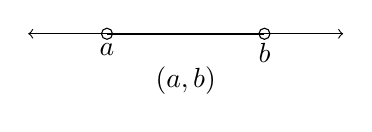
\begin{tikzpicture} %opið bil
\draw (0,0) circle (2pt) node[below] {$a$};
\draw (2,0) circle (2pt) node[below] {$b$};
\draw[<->] (-1,0) -- (3,0);
\node (c) at (1,-0.6) {$(a,b)$};
\draw[thick] (0,0)--(2,0);
\end{tikzpicture}

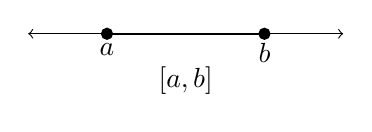
\begin{tikzpicture} %lokað bil
\filldraw[black] (0,0) circle (2pt) node[below] {$a$};
\filldraw[black] (2,0) circle (2pt) node[below] {$b$};
\draw[<->] (-1,0) -- (3,0);
\node (c) at (1,-0.6) {$[a,b]$};
\draw[thick] (0,0)--(2,0);
\end{tikzpicture}

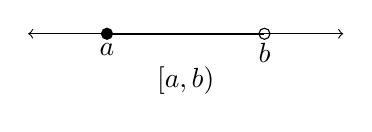
\begin{tikzpicture} %hálfopið bil 1
\filldraw[black] (0,0) circle (2pt) node[below] {$a$};
\draw (2,0) circle (2pt) node[below] {$b$};
\draw[<->] (-1,0) -- (3,0);
\node (c) at (1,-0.6) {$[a,b)$};
\draw[thick] (0,0)--(2,0);
\end{tikzpicture}

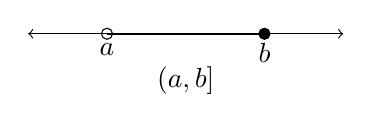
\begin{tikzpicture} %hálfopið bil 2
\draw (0,0) circle (2pt) node[below] {$a$};
\filldraw[black] (2,0) circle (2pt) node[below] {$b$};
\draw[<->] (-1,0) -- (3,0);
\node (c) at (1,-0.6) {$(a,b]$};
\draw[thick] (0,0)--(2,0);
\end{tikzpicture}

\end{document}
